%*****************************************
\chapter{Mixed Methods}\label{ch14:mixed}
%*****************************************

\begin{wrapfigure}{r}{0.4\textwidth}
	\centering
	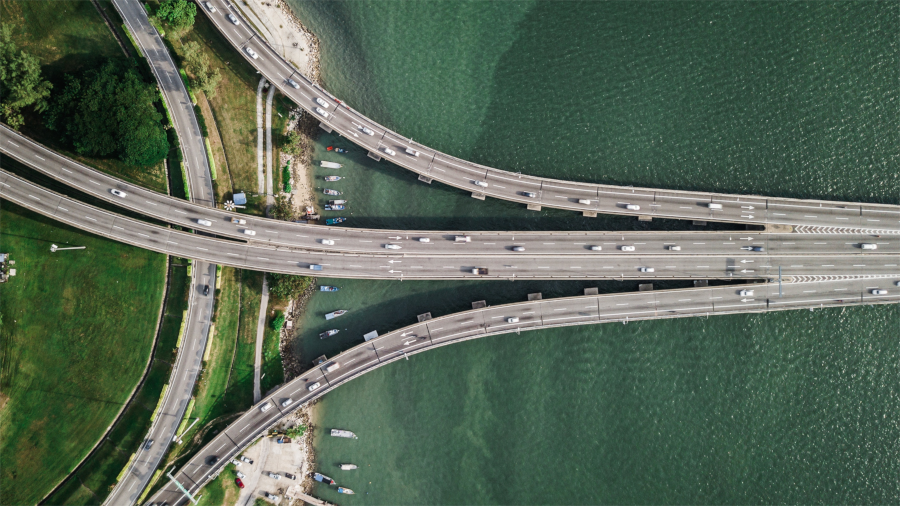
\includegraphics[width=0.4\textwidth]{gfx/14-intersection} 
\end{wrapfigure}

Often, researchers are not comfortable taking a single approach to a question and suspect that there is more to be discovered by looking at the question from multiple perspectives. In these cases, researchers may choose to use a second or even third approach to the research design in order to triangulate on a more satisfactory explanation for the question. Like two or three highways merging onto a single bridge, researchers can merge several methods into a single project.\blfootnote{Photo by Fahrul Azmi on Unsplash}

\begin{center}
	\begin{objbox}{Objectives}
		\begin{itemize}
			\setlength{\itemsep}{0pt}
			\setlength{\parskip}{0pt}
			\setlength{\parsep}{0pt}
			
			\item Describe the strengths and weaknesses of quantitative research methods.
			\item Describe descriptive and inferential techniques
			\item Describe the strengths and weaknesses of qualitative research methods.
			\item Define grounded theory and describe how grounded theory is developed.
			\item Compare and contrast quantitative and qualitative methods.
			\item Define mixed methods.
			\item Describe sequential explanatory, sequential exploratory, and convergent parallel research methods.
		\end{itemize}
	\end{objbox}
\end{center}

\section{Introduction}

There are, broadly speaking, two ways to approach a project: \gls{quantitativeresearch} and \gls{qualitativeresearch}. Quantitative research projects gather numeric data and analyze those data with statistical tools. Qualitative research projects gather non-numeric data and analyze those data with non-mathematical tools. It is possible, though, to combine both types of analysis in a single research project, a process known as \gls{mixedmethods}. This chapter first briefly revisits both quantitative and qualitative methods and then considers the process used to combine those methods.\footnote{This chapter is an expansion of information first presented in Chapter \ref{06:data}. Readers may want to review that material to help clarify concepts presented here.}

The following table is presented as a summary of the quantitative and qualitative research paradigms.

\begin{itemize}
	\item Quantitative Research
	\begin{itemize}
		\item \textbf{Philosophy}: positivism
		\item \textbf{Logic}: deductive
		\item \textbf{Focus}: counting and statistics
		\item \textbf{Epistemology}: objective point of view, researcher is separate from the observations
		\item \textbf{Causality}: phenomena have real causes
		\item \textbf{Data collection}: counting and measuring
		\item \textbf{Analysis}: statistical
	\end{itemize}
	\item Qualitative Research
	\begin{itemize}
		\item \textbf{Philosophy}: constructivism
		\item \textbf{Logic}: inductive
		\item \textbf{Focus}: interpreting observations
		\item \textbf{Epistemology}: subjective point of view, researcher and observations are inseparable
		\item \textbf{Causality}: All phenomena shape each other so it is impossible to distinguish causes from effects
		\item \textbf{Data collection}: observing and recording
		\item \textbf{Analysis}: grounded theory
	\end{itemize}
	
\end{itemize}

\section{Quantitative Analysis}

Numeric data collected in a research project can be analyzed quantitatively using statistical tools in two different ways. 

\begin{itemize}

	\item Descriptive analysis refers to statistically describing, aggregating, and correlating variables. 

	\item Inferential analysis refers to the statistical testing of hypotheses. 

\end{itemize}

\subsection{Quantitative Analysis: Descriptive}

\subsubsection{Univariate Analysis}

Univariate analysis, or analysis of a single variable, refers to a set of statistical techniques that can describe the general properties of one variable. Univariate statistics include: (1) frequency distribution, (2) central tendency, and (3) dispersion. 

\paragraph{Frequency Distribution} The frequency distribution of a variable is a summary of the frequency that individual values are found in a variable. For instance, it is easy to measure how often customers in a grocery store purchase types of products, like ``produce,'' ``dairy,'' and ``meat.'' If the number (or percentage) of observations within each category are counted and displayed in a table it would be called a \textit{frequency distribution}, as seen in Table \ref{14:tab01}. A frequency distribution can also be depicted in the form of a bar chart, as shown in Figure \ref{14:fig01}, with the horizontal axis representing number of purchases in each category and the vertical axis representing the categories.

\begin{table}[H]
	\rowcolors{1}{}{tablerow} % zebra striping background
	{\small
		%\fontsize{8}{10} \selectfont %Replace small for special font size
		\begin{longtable}{
				R{0.15\linewidth}
				C{0.15\linewidth}
			} %Left-aligned, Max width: 4.25in
			% \multicolumn{2}{c}{\textbf{Header 1}}\\
			\textbf{Item} & \textbf{Number} \endhead
			\hline
			Produce & $ 374 $ \\
			Dairy   & $ 291 $ \\
			Meat    & $ 187 $ \\
			\rowcolor{captionwhite}
			\caption{Frequency Table}
			\label{14:tab01}
		\end{longtable}
	} % End small
\end{table}

\vspace{.15in}

\begin{figure}[H]
	\centering
	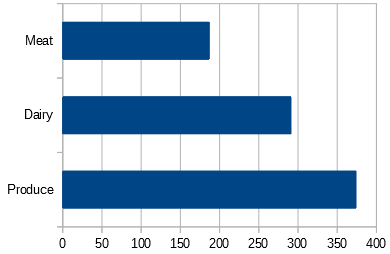
\includegraphics[width=\maxwidth{.95\linewidth}]{gfx/14-BarChart}
	\caption{Bar Chart}
	\label{14:fig01}
\end{figure}

\paragraph{Central Tendency} It is often desired to find the center of a data set and there are three commonly-used calculations: mean, median, and mode. 

\begin{enumerate}

	\item The arithmetic mean (often simply called the ``mean'') is the ``average'' of all values in a given distribution. This is the calculation most school children are taught and is found by adding all of the values together and dividing by the number of values.

	\item The median is the middle value in a distribution. This is computed by placing all of the values in order and selecting the one in the middle. In case there are two middle values (if there is an even number of values) then the median is the mean of the two middle values.
	
	\item The mode is the most frequently occurring value in a distribution of values. Mode is normally only used for categorical data rather than numeric. For example, if an item on a survey asked whether respondents rented, leased, or owned their office building it would not make sense to try to find an ``average'' for those values, instead the most frequently-selected response would be reported as the mode. 

\end{enumerate}

\paragraph{Dispersion} This refers to the way values are spread around the center of the data. Two common measures of dispersion are the range and standard deviation. 

\begin{enumerate}
	\item The range is the difference between the highest and lowest values in a distribution. The range is sensitive to the presence of outliers, which makes its use problematic. For instance, imagine that the values of the houses in a neighborhood were listed and they were all between $ \$100K $ and $ \$200K $ except one large house that was worth $ \$ 300K $. That one outlier value would make the range much larger than expected.

	\item The standard deviation is calculated by finding each value's distance from the mean of the data set (its deviation) and then finding the mean of all of those deviations. While the calculation is a somewhat complex, all statistics software packages are able to calculate the standard deviation. Because of the way it is calculated, the standard deviation is not sensitive to outliers so it is often used to indicate the data dispersion.

\end{enumerate}

\subsubsection{Bivariate Analysis}

Bivariate analysis examines how two variables are related to each other. The most common bivariate statistic is a correlation, which is a number between $ -1.00 $ and $ +1.00 $ denoting the strength and direction of the relationship between two variables. As an example, consider a data set that contains selected specifications found in the $ 1974 $ \textit{Motor Trend} magazine for $ 32 $ automobiles ($ 1973 $–$ 74 $ models)\footnote{The Motor Trend data was originally published in a report by Henderson and Vellerman in \textit{Biometrics}\cite{henderson1981building}.}. The first few items in that data set are shown in Table \ref{14:tab02}.

\begin{table}[H]
	\rowcolors{1}{}{tablerow} % zebra striping background
	{\small
		%\fontsize{8}{10} \selectfont %Replace small for special font size
		\begin{longtable}{
				L{0.20\linewidth}
				C{0.10\linewidth}
				C{0.05\linewidth}
				C{0.10\linewidth}
				C{0.05\linewidth}
				C{0.10\linewidth}
				C{0.10\linewidth}
			} %Left-aligned, Max width: 4.25in
			% \multicolumn{2}{c}{\textbf{Header 1}}\\
			\textbf{Name} & \textbf{mpg} & \textbf{cyl} & \textbf{disp} & \textbf{hp} & \textbf{wt} & \textbf{qsec}  \endhead
			\hline
			Mazda RX4      & $21.0$ & $6$ & $160$ & $110$ & $2.620$ & $16.46$ \\ 
			Datsun 710     & $22.8$ & $4$ & $108$ & $93$  & $2.320$ & $18.61$ \\ 
			Hornet 4 Drive & $21.4$ & $6$ & $258$ & $110$ & $3.215$ & $19.44$ \\ 
			Valiant        & $18.1$ & $6$ & $225$ & $105$ & $2.460$ & $20.22$ \\ 
			\rowcolor{captionwhite}
			\caption{Sample of Motor Trend Car Data}
			\label{14:tab02}
		\end{longtable}
	} % End small
\end{table}

Two of the variables in this data set are \textit{disp} (engine displacement) and \textit{qsec} (quarter-mile time, in seconds). It would be normal to expect that the greater the engine displacement (that is, the larger the engine) then the faster the automobile would finish a quarter-mile track. It turns out that the correlation between displacement and quarter-mile time is $ -0.43 $. The negative sign indicates that the relationship is negative, that is, as the displacement increases the time decreases. The magnitude of the correlation, though, indicates that this is not a particularly strong relationship, so a lot of small engines can finish the quarter-mile track as quickly as larger engines. A researcher would want to know why and one of the first confounding factors to consider would be the weight of the automobile. Are automobiles with larger engines also heavier, and, thus, slower through the quarter-mile?

Researchers can use a powerful visual aid to compare the correlations between numerous variables in a single data set using a correlation plot. Figure \ref{14:fig04} shows a correlation plot for each of the Motor Trend variables listed in Table \ref{14:tab02}.

\begin{figure}[H]
	\centering
	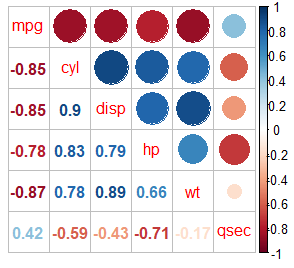
\includegraphics[width=\maxwidth{.95\linewidth}]{gfx/14-corplot}
	\caption{Correlation Plot}
	\label{14:fig04}
\end{figure}

In the correlation plot, the names of the variables are listed diagonally from the top left to the bottom right. In the lower half of the plot the correlations are reported numerically. Thus, the correlation between \textit{mpg} and \textit{cyl} is $ -0.85 $. Those correlations are also color-coded using the scale found on the right side of the plot. Since $ -0.85 $ is a fairly strong negative correlation it is printed in a dark red color. The top half of the plot shows the correlations using circles where both color and size indicate the strength and direction of the correlation. Thus, the correlation between \textit{wt} and \textit{qsec} is very weak since the size of the circle is small and it is negative since the color is pale pink. Using a correlation plot, researchers can very quickly locate strong positive and negative correlations, like \textit{mpg} and \textit{wt} (strong negative) or \textit{disp} and \textit{wt} (strong positive).

Another useful tool is a scatter plot. Consider Figure \ref{14:fig05}, which shows the relationship between the waiting time and eruption time for the \textit{Old Faithful} geyser in \textit{Yellowstone Park} \footnote{These data were first published by H{\"a}rdle in \textit{Smoothing Techniques with Implementation in S}\cite{hardle2012smoothing}.}. The plot clearly shows that the longer people have to wait for an eruption (time along the X-Axis increases) then the longer the eruption will last (time along the Y-Axis increases). This scatter plot also shows two clear groups of points so it would be reasonable to conclude that there are ``short'' eruptions and ``long'' eruptions.

\begin{figure}[H]
	\centering
	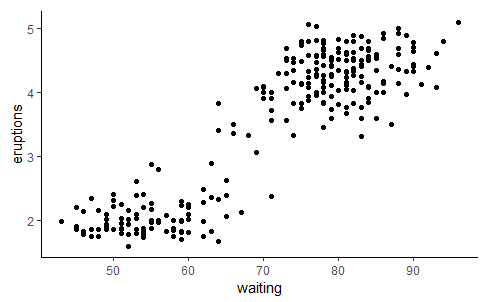
\includegraphics[width=\maxwidth{.95\linewidth}]{gfx/14-Faithful}
	\caption{Scatter Plot}
	\label{14:fig05}
\end{figure}

\subsection{Quantitative Analysis: Inferential}

Inferential statistics are procedures used to reach conclusions about the associations between variables. They differ from descriptive statistics in that they are explicitly designed to test a hypothesis. Numerous statistical procedures fall in this category but all are supported by statistical software like \textit{R}. This chapter provides only a short primer on the most basic and frequent inferential procedures. First, though, it is important to define \textit{hypothesis}.

\subsubsection{Definition of Hypothesis}

A hypothesis is a proposition put forth to explain some observed phenomena. Often, a hypothesis also functions in a predictive manner and is capable of being tested by scientific methods. For example, a researcher might hypothesize that ads placed in a local newspaper are more effective than those placed on a local radio station. This hypothesis could then be tested by placing ads in both media and measuring the results of those ads. An hypothesis typically has these characteristics:

\begin{itemize}
	\item Clear. The hypothesis must be stated in clear and precise language.
	\item Testable. A hypothesis must be testable with some way to determine if the hypothesis is true or false.
	\item Consistent. A hypothesis should be consistent with known facts or an established body of literature.
	\item Timely. A hypothesis must be able to be confirmed (or rejected) in a reasonable time frame.
\end{itemize} 

It is normally not possible to actually prove a hypothesis since it is not possible to analyze all possible relevant data. In the case of the advertising media mentioned above, it would not be possible to prove that hypothesis for every possible combination of newspaper and radio ads, in all possible markets, in all possible seasons, for all possible products. Thus, research projects normally include both a \textit{Null Hypothesis} and an \textit{Alternative Hypothesis}. The alternative hypothesis is an attempt to explain some phenomena while the null hypothesis, generally, states that the explanation is wrong. For example, consider this hypothesis and its null:

\begin{description}
	\item[Alternative] Ads placed in a local newspaper are more effective than those placed on a local radio station.
	\item[Null] The type of media does not change the effectiveness of an ad.
\end{description}

Normally, the alternative hypothesis cannot be proven, or even tested, directly; rather, its veracity is determined by rejecting (or not) the null hypothesis. For example, if a merchant ran ads in a newspaper and on the radio and it seemed like the newspaper ads were more effective, would this verify the hypothesis or is the result nothing more than dumb luck? Statistically, the probability that a conclusion is caused by mere chance is called the \textit{p-value} (for ``probability value''). At the onset of a project, researchers determine the maximum acceptable probability that the project's conclusion is \textit{in}correct. Most business and marketing research uses a \textit{p-value} of $ 0.05 $ (or $ 5\% $) as the cutoff. Thus, a calculated \textit{p-value} that is less than $ 0.05 $ indicates that the null hypothesis can be rejected but if the \textit{p-value} is greater than $ 0.05 $ then the null hypothesis cannot be rejected. All statistics programs, like \textit{R}, automatically calculates a \textit{p-value} as part of the output for many statistical tests.

\subsubsection{Comparing Two Groups}

One of the simplest inferential analyses is comparing the outcomes of treatment and control groups; for example, determining whether students enrolled in an ``enhanced'' mathematics program perform better than those in a traditional program. In this case, the measured outcome variable could be a standardized test score following the mathematics courses. The analytic technique for this simple design is a \textit{t-test}.\footnote{The \textit{t-test} was introduced in $ 1908 $ by William Sealy Gosset, a chemist working for the Guiness Brewery in Dublin, Ireland, to monitor the quality of stout --- a dark beer popular with nineteenth-century porters in London. Because his employer did not want to reveal the fact that it was using statistics for quality control, Gosset published the test in \textit{Biometrika} using his pen name ``Student.'' The test involved calculating the value of ``t,'' which was a letter used frequently to denote the difference between two groups. Hence, the name ``Student's t-test.''}

The t-test examines whether the means of two groups are statistically different from each other (non-directional or two-tailed test), or whether one group has a statistically larger (or smaller) mean than the other (directional or one-tailed test). In the mathematics example, if the goal is to examine whether students in the enhanced mathematics program perform better than those in a traditional program it would be a one-tailed test. The hypothesis can be stated as:

\begin{description}
	\item[Alternate] The enhanced program scores are greater than the traditional program scores.
	\item[Null] The enhanced program scores are not greater than the traditional program scores.
\end{description}

Note that the goal of a statistical significance test is to reject the null hypothesis---in other words, to show that there is a difference between the two groups being compared. If a t-test is run on the outcome scores for the two mathematics programs it would produce a \textit{p-value} (among other things) and if that value is less than $ 0.05 $ then researchers can assume that the means are truly different and then reject the null hypothesis.

Extending the mathematics program example, imagine that the hypothesis is changed a bit such that the amount of instructional time, either three or six hours/week, is also considered. This creates what is called a $ 2 x 2 $ factorial design, with the two factors being program type (enhanced vs. traditional) and instructional time (three vs. six hours/week). This type of design helps researchers estimate the independent effect of each factor, called \textit{main effects}, but also the joint effect of both factors, called the \textit{interaction effect}. This type of factorial design can be analyzed using a two-way \textit{ANOVA}; but, again, researchers would look for a \textit{p-value} less than $ 0.05 $ to indicate which factors were significant.

\subsubsection{Other Quantitative Analysis}

Following are a few other inferential statistical techniques that are sometimes found in research reports.

\begin{itemize}
	\item \textbf{Factor analysis} is a data reduction technique that is used to statistically aggregate a large number of observed measures (items) into a smaller set of unobserved (latent) variables called factors based on their underlying bi-variate correlation patterns. As an example, perhaps a researcher could aggregate income, home value, and tax bracket into a single factor named ``wealth.''

	\item \textbf{Discriminant analysis} is a classification technique that aims to place a given observation in one of several nominal categories based on a linear combination of predictor variables. It is popular in marketing applications, such as for classifying customers or products into categories based on salient attributes as identified from large-scale surveys.

	\item \textbf{Logistic regression} is a model in which the outcome variable is binary (zero or one) and is presumed to follow a logistic distribution. The goal of the regression analysis is to predict the probability of the successful outcome by fitting data into a logistic curve. An example is predicting the probability of heart attack within a specific period, based on predictors such as age, body mass index, exercise regimen, and so forth. Logistic regression is extremely popular in the medical sciences. 

	\item \textbf{Probit regression} is a model in which the outcome variable can vary between zero and one and is presumed to follow a standard normal distribution. The goal of the regression is to predict the probability of each outcome. This is a popular technique for predictive analysis in the actuarial science, financial services, insurance, and other industries for applications such as credit scoring based on a person's credit rating, salary, debt and other information from a loan application.

	\item \textbf{Path analysis} is a technique for analyzing directional relationships among a set of variables. It allows for examination of complex models where the dependent variable in one equation is the independent variable in another equation, and is widely used in contemporary social science research. As an example, perhaps a project shows that disposable income is dependent on age (that is, as people age they tend to have more disposable income), then that disposable income becomes the independent variable in a follow-on study to determine if there is a relationship between income and happiness.

	\item \textbf{Time series analysis} is a technique for analyzing time series data, or variables that continually changes with time. Examples of applications include forecasting stock market fluctuations and urban crime rates. This technique is popular in econometrics, mathematical finance, and signal processing.
	
\end{itemize}

\section{Qualitative Analysis}

Qualitative analysis is the analysis of qualitative data such as text data from interview transcripts. Unlike quantitative analysis, which is statistics driven and largely independent of the researcher, qualitative analysis is heavily dependent on the researcher's analytic skills and knowledge of the social context from where the data are collected. The emphasis in qualitative analysis is ``sense making'' or understanding a phenomenon rather than predicting or explaining. A creative and investigative mindset is needed for qualitative analysis along with a set of analytic strategies. 

\subsection{Grounded Theory}

How is a vast set qualitative data acquired through participant observation, in-depth interviews, focus groups, or other narratives analyzed? One technique is \gls{groundedtheory}, which is a technique of interpreting data about a social phenomenon with a goal of building theories. The technique was developed by Glaser and Strauss\cite{glaser1967discovery} in their method of constant comparative analysis of grounded theory research, and refined by Corbin and Strauss\cite{corbin1990grounded} to further illustrate specific coding techniques---a process of classifying and categorizing text data segments into a set of codes, categories, and relationships. The interpretations are ``grounded in'' (or based on) observed empirical data, hence the name. Strauss and Corbin\cite{strauss1998basics} describe the following three coding techniques for analyzing text. 

\begin{description}

\item[Open coding] is designed to identify key ideas in the textual data that are related to the phenomenon of interest. The researcher examines the raw textual data line by line to identify events, incidents, ideas, actions, perceptions, and interactions of relevance, which are coded as ``concepts.'' Each concept is linked to specific portions of the text (coding unit) for later validation. Some concepts may be simple, clear, and unambiguous while others may be complex, ambiguous, and viewed differently by different participants. The coding unit may vary with the concepts being extracted. Simple concepts such as ``organizational size'' may include just a few words of text, while complex ones such as ``organizational mission'' may span several pages. Concepts can be named using the researcher's own naming convention or standardized labels taken from the research literature. Once a basic set of concepts are identified they can be used to code the remainder of the data while continuing to look for new concepts. While coding, it is important to identify the recognizable characteristics of each concept, such as its size, color, or level (\eg, high or low), so that similar concepts can later be grouped together. This coding technique is called ``open'' because the researcher is open to new concepts relevant to the phenomenon of interest.

\item[Axial coding] groups concepts into higher order categories. While concepts may be context-specific, categories tend to be broad and generalizable and ultimately evolve into constructs in a grounded theory. Categories are needed to reduce the amount of concepts the researcher must work with and to build a ``big picture'' of the issues salient to understanding the phenomenon under consideration. Constructs from the existing literature can be used to name these categories, particularly if the goal of the research is to extend current theories. The characteristics (properties) and dimensions of each category should be identified. The dimension is a value of a characteristic along a continuum. For example, a ``communication media'' category may have a characteristic called ``speed,'' which can be dimensionalized as fast, medium, or slow. The relationships between categories may be clearly evident or subtle. In the latter instance, researchers may use a coding scheme to understand which categories represent conditions (the circumstances in which the phenomenon is embedded), actions/interactions (the responses of individuals to events under these conditions), and consequences (the outcomes of actions/ interactions). As conditions, actions/interactions, and consequences are identified, theoretical propositions start to emerge, and researchers can start explaining why a phenomenon occurs, under what conditions, and with what consequences.

\item[Selective coding] involves identifying a central category or core variable and systematically and logically relating this central category to other categories. The central category can evolve from existing categories or can be a higher order category that subsumes previously coded categories. New data are selectively sampled to validate the central category and its relationships to other categories (\ie, the tentative theory). Selective coding limits the range of analysis and makes it move faster than open and axial coding.

\end{description}

During the coding process, the coder be alert for categories that may emerge from new data that are related to the phenomenon of interest. Hence, open, axial, and selective coding often proceed simultaneously. Coding of new data and theory refinement continues until theoretical saturation is reached, \ie, when additional data does not yield more than marginal change in the core categories or the relationships.

The ``constant comparison'' process implies continuous rearrangement, aggregation, and refinement of categories, relationships, and interpretations based on increasing depth of understanding, and an iterative interplay of the following four stages of activities:

\begin{enumerate}
	\item comparing incidents/texts assigned to each category (to validate the category)
	\item integrating categories and their properties
	\item delimiting the theory (focusing on the core concepts and ignoring less relevant concepts)
	\item writing theory
\end{enumerate}

After a grounded theory is generated, it must be refined for internal consistency and logic. Researchers must ensure that the central construct has the stated characteristics and dimensions, and if not, the data analysis may be repeated. Researcher must then ensure that the characteristics and dimensions of all categories show variation. For example, if behavior frequency is one such category, then the data must provide evidence of both frequent performers and infrequent performers of the focal behavior. Finally, the theory must be validated by comparing it with raw data. If the theory contradicts observed evidence then the coding process may be repeated to reconcile such contradictions or unexplained variations. 

\section{Quantitative vs. Qualitative}

Given their differences, it may come as no surprise that quantitative and qualitative research do not coexist in complete harmony. Some quantitative researchers criticize qualitative methods on the grounds that they lack objectivity, are difficult to evaluate in terms of reliability and validity, and do not allow generalization to people or situations other than those actually studied. At the same time, some qualitative researchers criticize quantitative methods on the grounds that they overlook the richness of human behavior and experience and instead answer simple questions about easily quantifiable variables.

In general, however, qualitative researchers are well aware of the issues of objectivity, reliability, validity, and generalizability. In fact, they have developed a number of frameworks for addressing these issues. Also, in general, quantitative researchers are well aware of the issue of oversimplification. They do not believe that all human behavior and experience can be adequately described in terms of a small number of variables and the statistical relationships among them. Instead, they use simplification as a strategy for uncovering general principles of human behavior.

\section{Combining Quantitative and Qualitative}

Quantitative research based on \gls{positivism} has historically been the cornerstone of business and marketing research. Purists call for researchers to ``eliminate their biases, remain emotionally detached and uninvolved with the objects of study and test or empirically justify their stated hypotheses''\cite{johnson2004mixed}.

Qualitative research is based on \gls{interpretivism} and its practitioners ``contend that multiple-constructed realities abound, that time- and context free generalizations are neither desirable nor possible, that research is value-bound, that it is impossible to differentiate fully causes and effects, that logic flows from specific to general and that knower and known cannot be separated because the subjective knower is the only source of reality''\cite{johnson2004mixed}.

It was in the 1980s and 1990s that researchers began to call for a ``truce'' in the ``Paradigm Wars'' between quantitative and qualitative methods. Many major authors and researchers felt that the two research methodologies are compatible and could be combined in a single research project. In fact, the proverbial pendulum has swung the other direction and many researchers now believe that there is no major problem area that should be studied exclusively with one research method. They believe that quantitative research answers the ``if'' question while qualitative research answers the ``how or why.'' This research paradigm is known as a \gls{mixedmethods} approach, though other phrases, like ``multi-modal,'' are occasionally used.

%TODO from Lorenzini
Mixed-method research offers powerful tools to investigate complex systems and processes in business, marketing, and economics. This method includes all phases of a research project, including philosophical assumptions, research questions, design, collection, analysis, integration and presentation of data and results. \footnote{The material in this section is adapted from Lorenzini, \textit{Mixed-Method Research in the Health Sciences}\cite{lorenzini2017mixed}}

The nature of the research question guides the selection of the method. Researchers in business-related fields use a quantitative methodology to study and answer research questions on causality, generalization, and magnitude of effect. The qualitative methodology is the choice of researchers who seek to answer research questions that explore how or why a given phenomenon occurs, to develop a theory, or describe the subjectivity of an individual experience.

Mixed-method research attempts to utilize the strengths of each of the two approaches, quantitative and qualitative, and, for this reason, it is being increasingly used to address contemporary research problems. An indication of the increased interest of this method was the publication of guidelines on mixed-methods research in various fields, like information systems\cite{venkatesh2013bridging} and health sciences\cite{creswell2004designing}.

Over the course of the years, several definitions of mixed methods have emerged but researchers seem to be focused on defining mixed-methods by its characteristics, which are\ldots

\begin{itemize}
	
	\item the collection and analysis of both quantitative and qualitative data takes place;

	\item rigorous procedures are used to carry out quantitative and qualitative research;

	\item there is integration or combination of results;

	\item procedures are developed in which data collection, analysis, and integration takes place.

\end{itemize}

It is often argued that the quantitative approach is not able to capture what is understood about the context where the study took place but qualitative research compensates for these weaknesses. On the other hand, qualitative research is seen as deficient due to the personal interpretations made by the researcher, the bias created because of this, the small number of participants, and the difficulty to generalize the results. Quantitative research, in turn, does not have those weaknesses. By using mixed methods, researchers can use all available tools rather  than confining themselves to data collection strategies commonly associated with either quantitative or qualitative research. 

\subsection{Triangulation}

One of the most commonly-used mixed methods tools is called ``triangulation.'' This term comes from old navigation methods where ships' captains could pinpoint their location by ``shooting an azmuth'' to two different visible points and then drawing intersecting lines on a map. In mixed methods research, triangulation is the process of using multiple sources to pinpoint a solution. Tashakkori\cite{tashakkori1998mixed} discusses four types of triangulation: data triangulation (the use of a variety of data sources in a study), investigator triangulation (the use of several different researchers), theory triangulation (the use of multiple perspectives to interpret the results of a study), and methodological triangulation (the use of multiple methods to study a research problem). Triangulation was the solution that broke the ``Paradigm Wars'' and permitted mixed methods research to begin to be accepted by scholars.

\subsection{Steps For Design}

While every research project is different, Venkatesh\cite{venkatesh2013bridging} created a six-step process for mixed methods research. While this process may need to be modified for specific projects, it is a good general-purpose start.

\begin{enumerate}
	\item Decide on the appropriateness of a mixed methods approach. Not every research project will benefit from a mixed methods approach. Consider things like the research question, purpose of the research project, and the selection of available paradigms. Keep in mind that a mixed methods project is more time and resource intensive so it would be too much for a simple project.
	\item Develop strategies for the design. There are three prevailing mixed method strategies (covered below) and once the decision is made to use a mixed methods procedure then it is time to determine the strategy to use. This decision is informed by what approaches of the project (qualitative or quantitative) will be completed first, the priority of approaches, how the data and results will be mixed, and the amount of time and expertise that is available.
	\item Develop strategies for collecting and analyzing data. Because the project will be completed in two phases (qualitative and quantitative) it is important to plan how to collect and analyze the data. Mistakes made in the first collection phase may not become evident until the second phase and that could sink the entire project.
	\item Draw meta-inferences from the results. This step is similar to developing a theory that explains the data and analysis. The information about grounded theory (above) may help with this step of the process.
	\item Assess the quality of the meta-inferences. The meta-inferences may be strong or weak. If they are weak then perhaps they need to be reconsidered or maybe the entire research project needs to be redone with appropriate changes to the protocol.
	\item Discuss potential threats and remedies. All research projects develop threats and it is important for the researcher to honestly approach those threats and propose remedies for them.
\end{enumerate}

\subsection{Strategies}

Mixed-methods projects typically fall into one of three general strategies, listed below and more fully described later in this chapter.\footnote{Tashakkori\cite{tashakkori1998mixed} identifies eight different strategies while Bryman and Bell\cite{bell2015business} lists nine strategies. The three listed in this chapter are from Creswell\cite{creswell2014research} and seem to be those most commonly cited in the literature.}

\begin{itemize}

	\item Sequential Explanatory

	\item Sequential Exploratory

	\item Convergent Parallel (Triangulation)

\end{itemize}

The specific type of strategy that is best for any given research project depends on the following four factors.

\begin{enumerate}
	\item Theoretical perspective of the researcher
	\begin{itemize}
		\item Explicit–--Does the researcher base the research project directly on a theory?
		\item Implicit–--Does the researcher only indirectly use theory as a foundation for the research project?
	\end{itemize}

	\item Priority of strategy
	\begin{itemize}
		\item Qualitative---Is the qualitative portion of the research project more important?
		\item Quantitative---Is the quantitative portion of the research project more important?
		\item Equal---Are the two types of research, quantitative/qualitative, equally used in the research project?
	\end{itemize}

	\item Sequence of data collection implementation
	\begin{itemize}
		\item Is the qualitative part completed first followed by the quantitative part?
		\item Is the quantitative part completed first followed by the qualitative part?
		\item Are both parts completed simultaneously?
	\end{itemize}

	\item The point at which the data are integrated
	\begin{itemize}
		\item At data collection
		\item At data analysis
		\item At data interpretation
		\item With some combination
	\end{itemize}

\end{enumerate}

\subsubsection{Sequential Explanatory Strategy}

The sequential explanatory strategy is used when a researcher already has a theory to explain some phenomena and wants to collect data to explain certain facets of that theory. Figure \ref{14:fig90} illustrates the process of a sequential explanatory strategy. 

\begin{figure}[H]
	\centering
	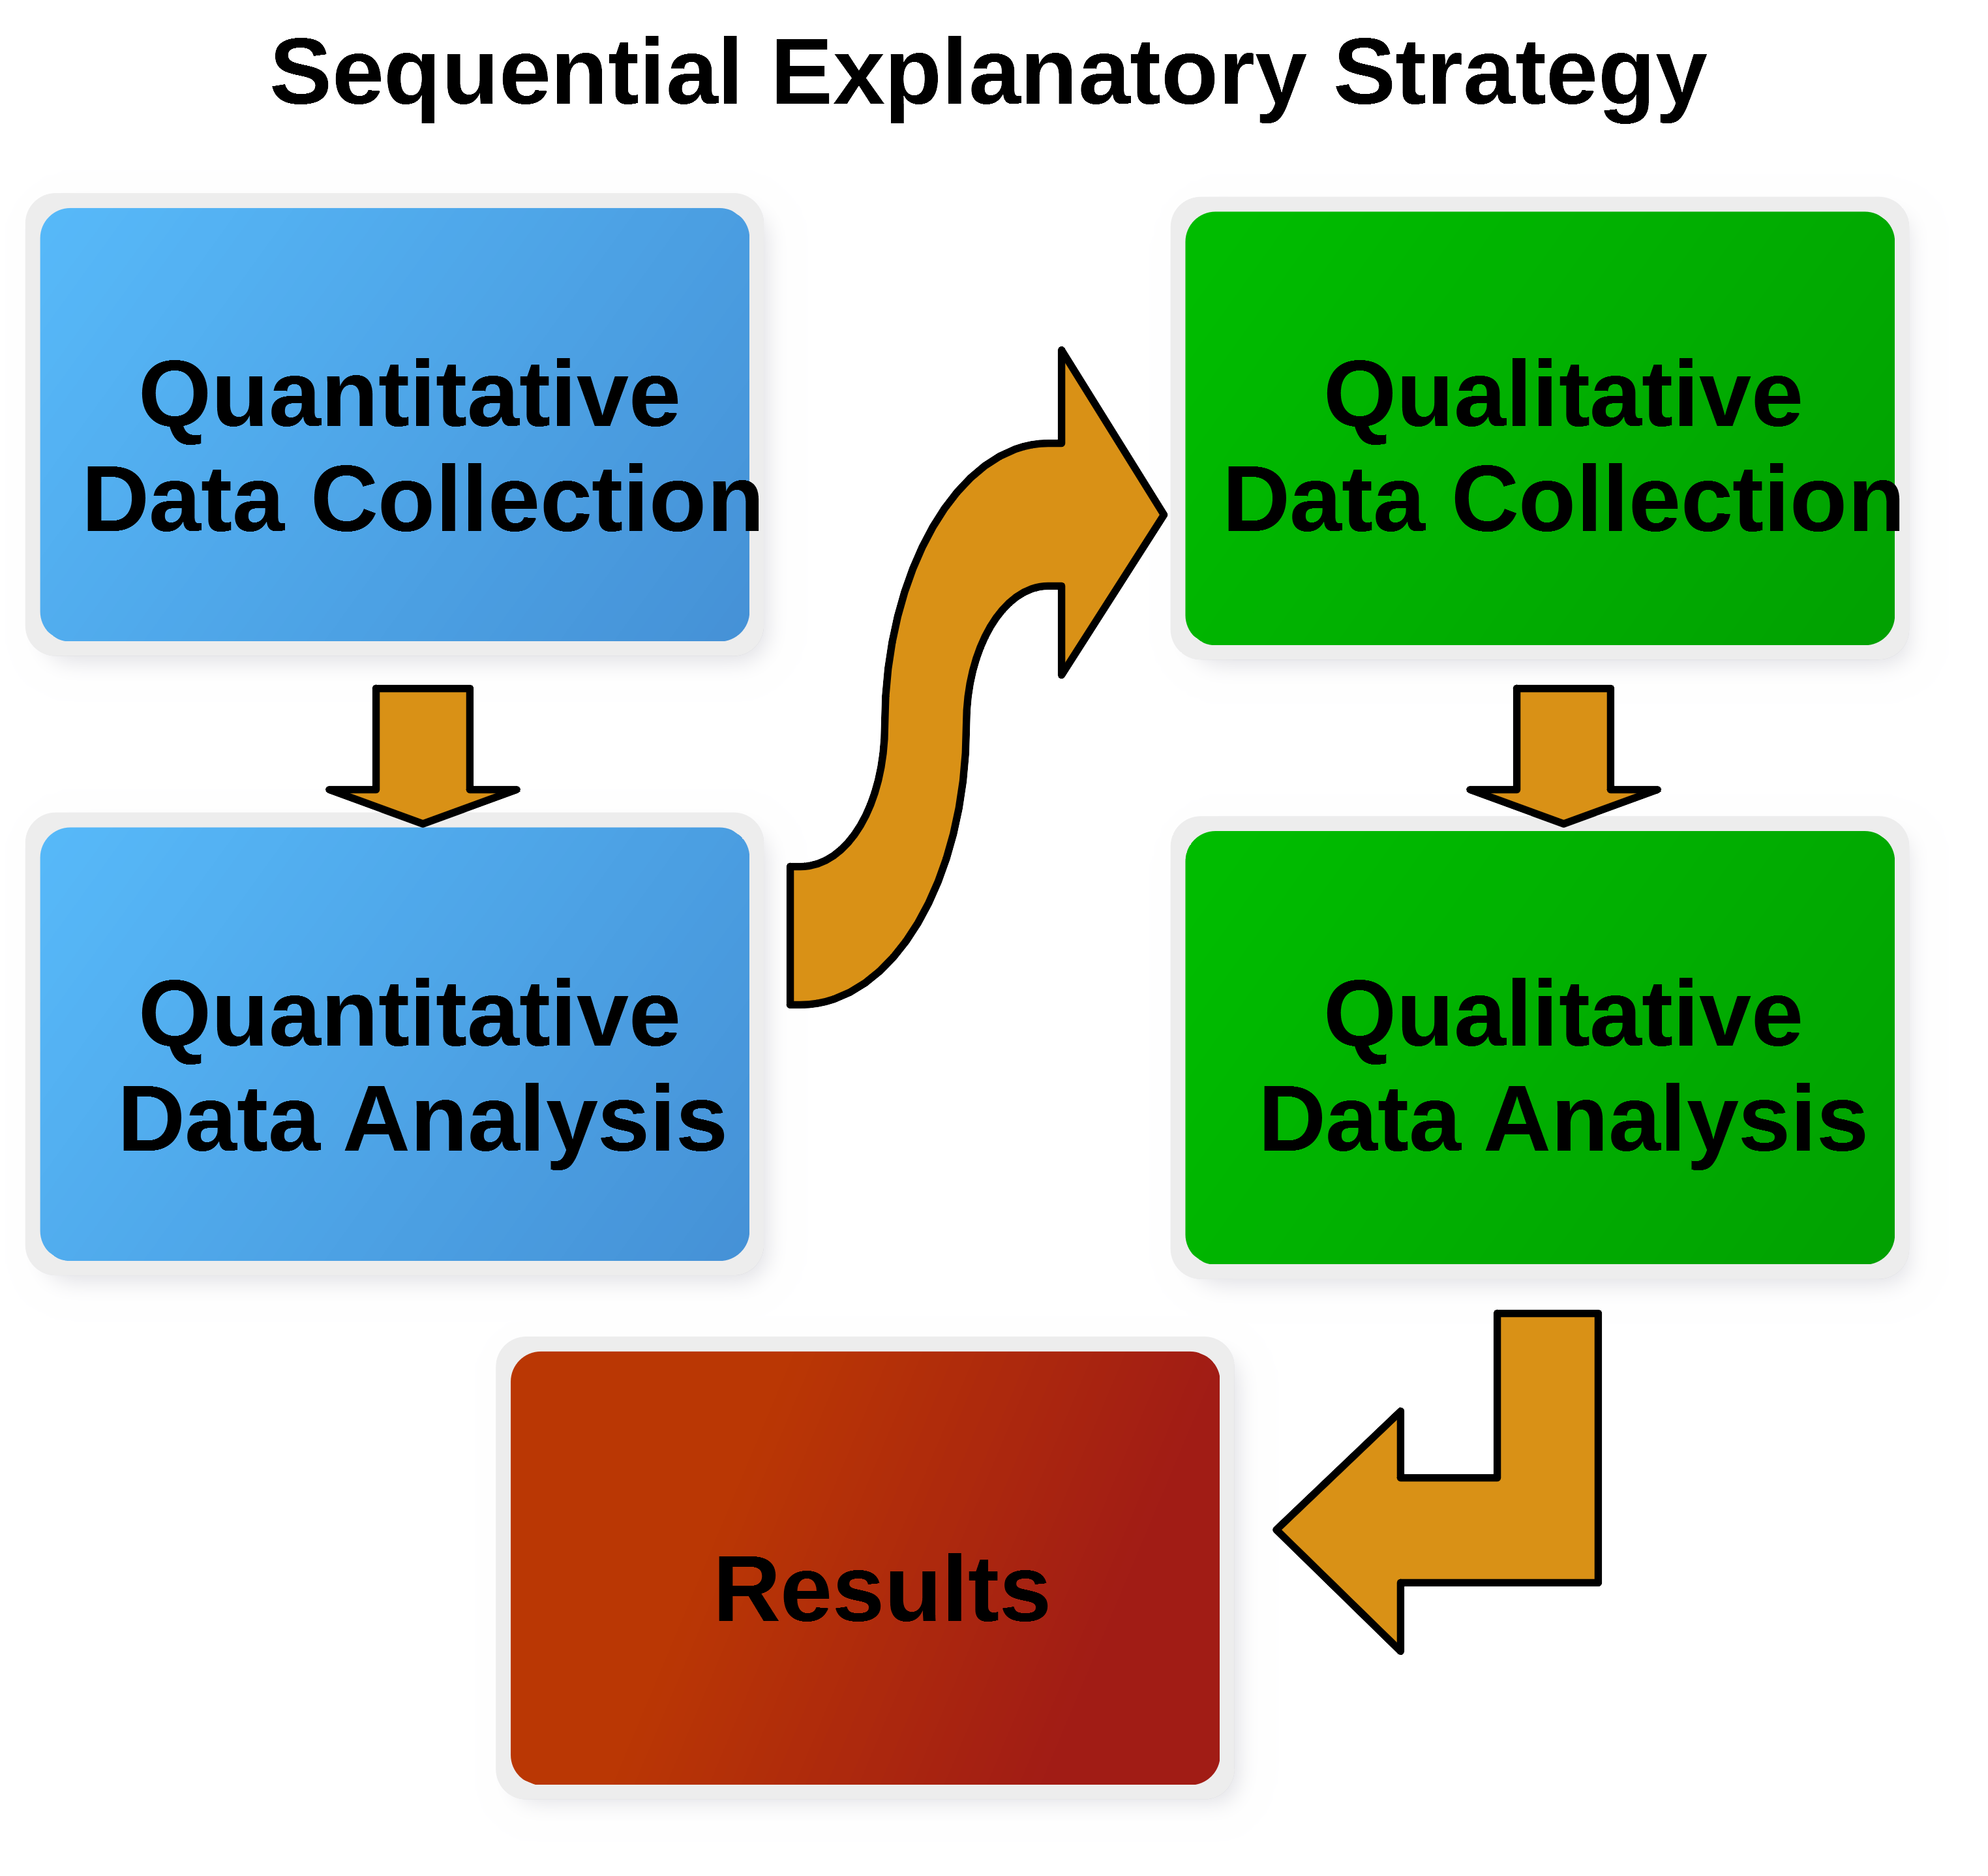
\includegraphics[width=\maxwidth{.95\linewidth}]{gfx/14-Seq_Explain}
	\caption{Sequential Explanatory}
	\label{14:fig90}
\end{figure}

The collection and analysis of quantitative data are followed by the collection and analysis of qualitative data where equal priority is given to the two phases. The data are integrated in the results phase. The primary focus of this strategy is to explain quantitative results by exploring those results in more detail or to help explain unexpected results (e.g., using follow-up interviews to better understand the results of a quantitative study).

\begin{description}
	\item[Strength]---relatively straightforward due to clear, distinct stages and easier to describe than concurrent strategies.

	\item[Weakness]---very time consuming especially when both phases are given equal consideration and priority.
\end{description}

\subsubsection{Sequential Exploratory Strategy}

The sequential exploratory strategy is used when a researcher is seeking to develop a theory related to some observation. Figure \ref{14:fig91} illustrates the process of a sequential exploratory strategy. 

\begin{figure}[H]
	\centering
	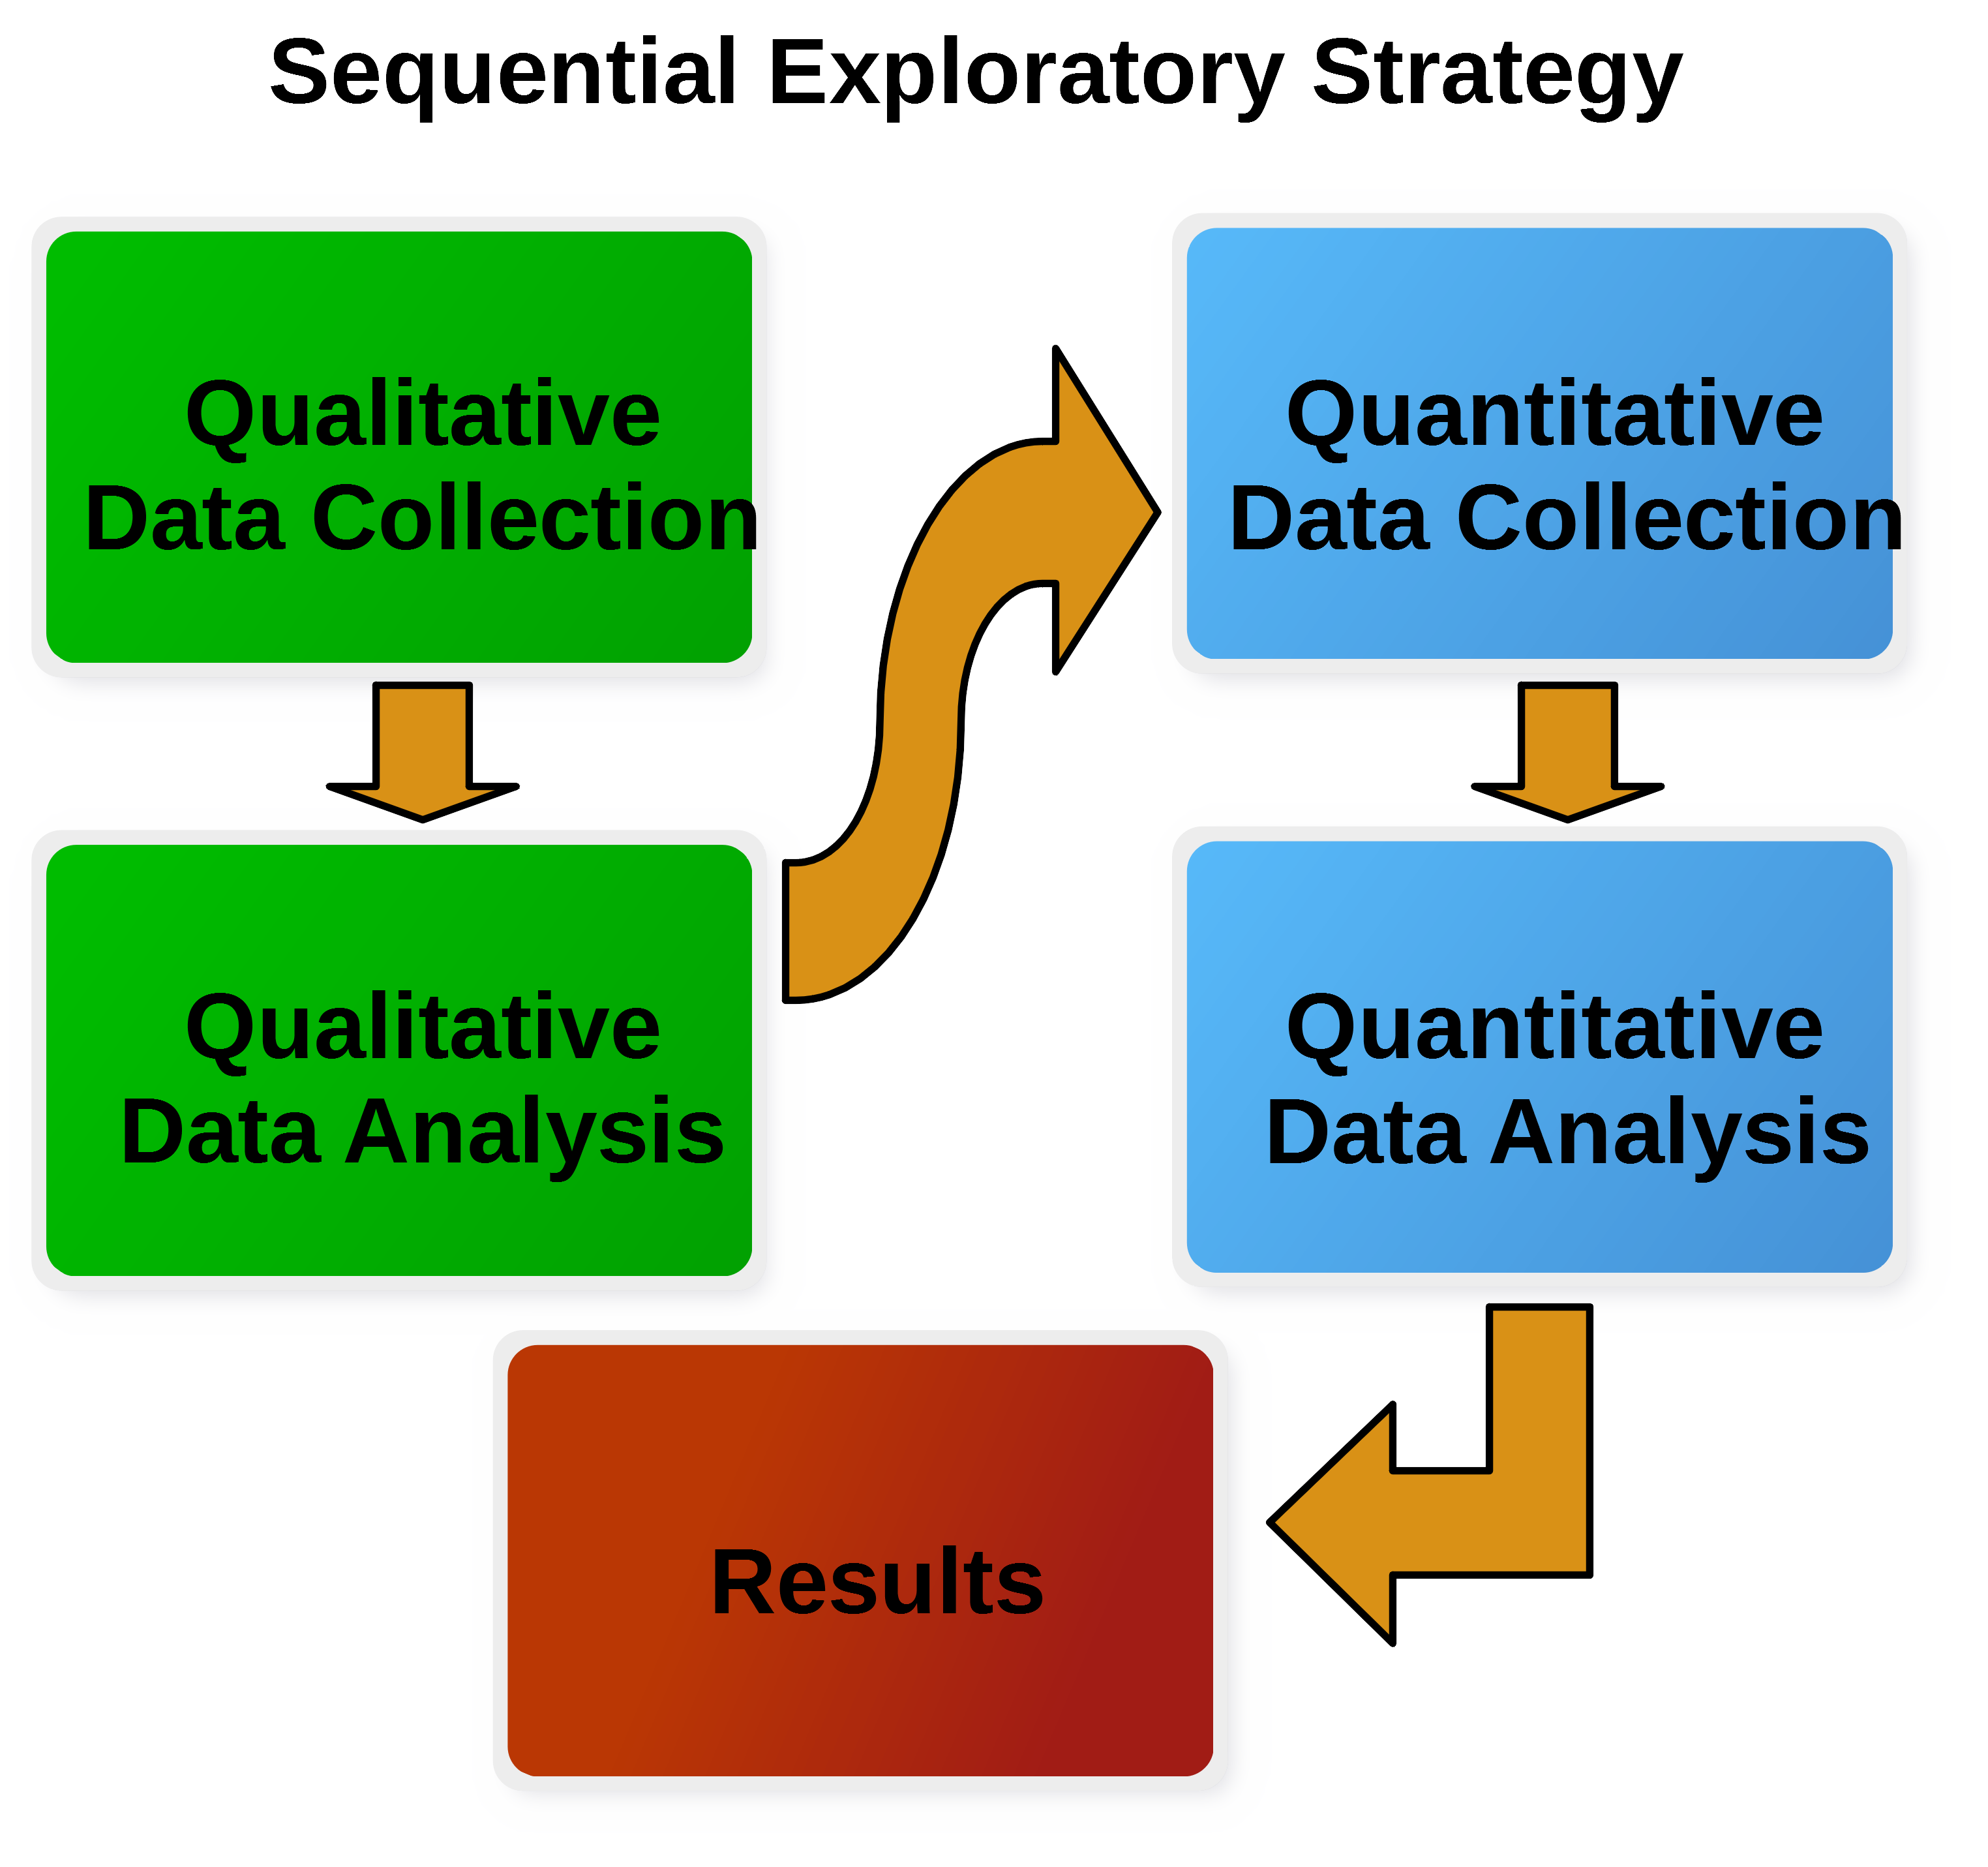
\includegraphics[width=\maxwidth{.95\linewidth}]{gfx/14-Seq_Explore}
	\caption{Sequential Exploratory}
	\label{14:fig91}
\end{figure}

The collection and analysis of qualitative data are followed by the collection and analysis of quantitative data where equal priority is given to the two phases but priority can be given to either as the project unfolds. Data are integrated during results phase. This strategy is used primarily to explore a phenomenon by testing the elements of a theory, generalizing qualitative findings to different samples, and the development of instrumentation (e.g., using a small group to create some sort of instrument, like a survey, and then collecting quantitative data based on that instrument).

\begin{description}
	\item[Strength]---relatively straightforward due to clear, distinct stages and easier to describe than concurrent strategies.
	\item[Weakness]---very time consuming, especially when both phases are given equal consideration and priority.
\end{description}

\subsubsection{Convergent Parallel (Triangulation)}

The convergent parallel strategy, often called ``triangulation,'' is used when a researcher is seeking to validate a research project by converging two, or more, research processes on a single observation. Figure \ref{14:fig92} illustrates the process of a convergent parallel strategy. 

\begin{figure}[H]
	\centering
	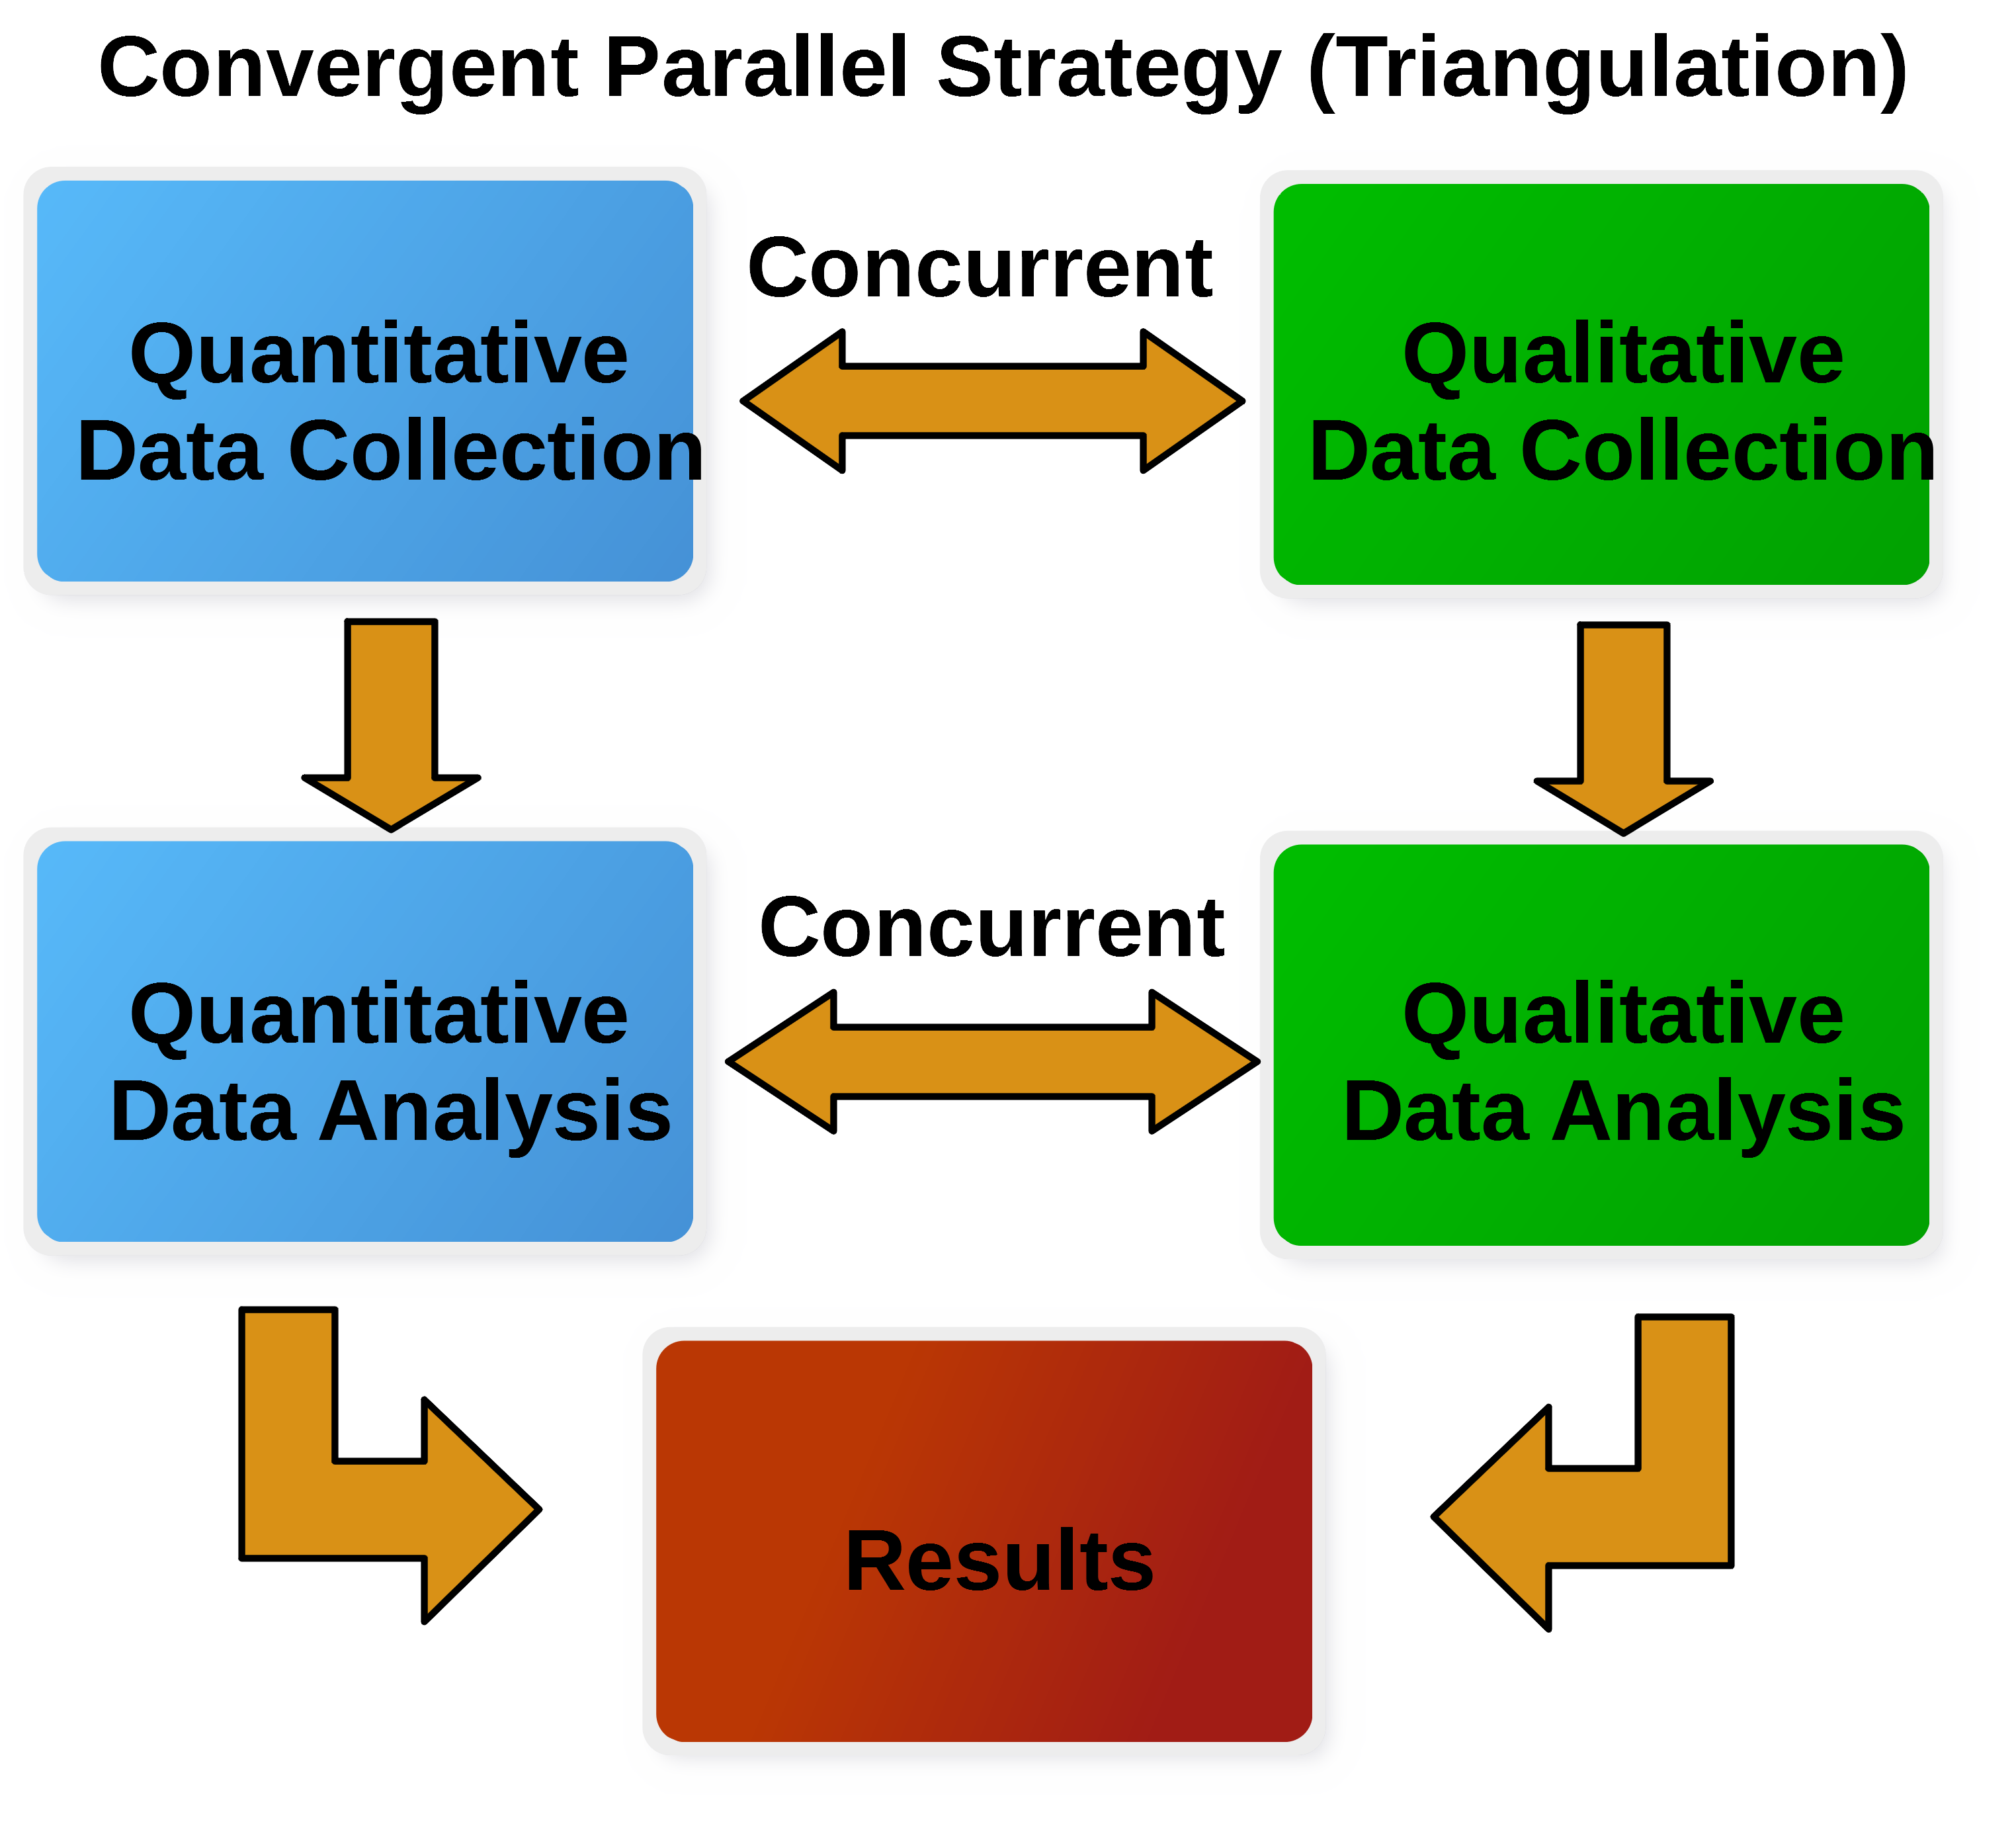
\includegraphics[width=\maxwidth{.95\linewidth}]{gfx/14-Triangulation}
	\caption{Triangulation}
	\label{14:fig92}
\end{figure}

There are two concurrent data collection phases where priority should be equal but can be shifted to either approach as necessary. Data are integrated during all phases. The results note any sort of convergence that strengthens knowledge claims, or, conversely, a lack of convergence that would tend to disprove the knowledge claims. It is primarily used for confirmation, corroboration or cross-validation within a single study.

\begin{description}
	\item[Strength]---familiar to many researchers. Shorter data collection time when compared to sequential methods. Offsets weaknesses inherent to one design by using both.
	\item[Weakness]---requires a great deal of expertise and effort to study the phenomenon under consideration using two different methods. It may be difficult to compare two types of data as well as resolve discrepancies if they arise.
\end{description}

\subsection{Mixed Method Strengths and Weaknesses}

Like any research paradigm, mixed methods has both strengths and weaknesses.\footnote{The strengths and weaknesses in this chapter are based on ``Demystifying Mixed Methods Research Design: A Review of the Literature'' by Gail D. Caruth\cite{caruth2013demystifying}}

\paragraph{Strengths} of the mixed method design include: 

\begin{itemize}
	\item they point out that words, photos, and narratives can be used to add meaning to numbers while numbers can add precision to words, photos, and narratives
	\item they can handle a wider range of research questions because the researcher is not limited to one research design
	\item they can present a more robust conclusion
	\item they offer enhanced validity through triangulation (cross validation)
	\item they can add insight and understanding that might be missed when only a single research design is used
	\item they can increase the capability to generalize the results compared to using only qualitative study designs
\end{itemize}

\paragraph{Weaknesses} of the mixed method design include: 

\begin{itemize}
	\item they can be difficult for a single researcher especially when the two designs are best used concurrently, in this case the study might require a research team
	\item they can be more time consuming and expensive when concurrency is involved
	\item they require that the researcher(s) learn multiple methods to combine them knowledgeably, defend the use of multiple methods, utilized them professionally, etc.
	\item they are not without conflict because methodological purists maintain that researchers should work within either a quantitative or a qualitative research design never mixing the two designs in a single study
\end{itemize}

\section{Key Takeaways}

\begin{center}
	\begin{tkawybox}{Mixed Methods}
		\begin{itemize}
			\setlength{\itemsep}{0pt}
			\setlength{\parskip}{0pt}
			\setlength{\parsep}{0pt}
			
			\item Describe the strengths and weaknesses of quantitative research methods.
			\item Describe descriptive and inferential techniques
			\item Describe the strengths and weaknesses of qualitative research methods.
			\item Define grounded theory and describe how grounded theory is developed.
			\item Compare and contrast quantitative and qualitative methods.
			\item Define mixed methods.
			\item Describe sequential explanatory, sequential exploratory, and convergent parallel research methods.
		\end{itemize}
	\end{tkawybox}
\end{center}
